\documentclass[border=10pt]{standalone}
\usepackage{pgfplots}
\pgfplotsset{compat=1.18}
\begin{document}
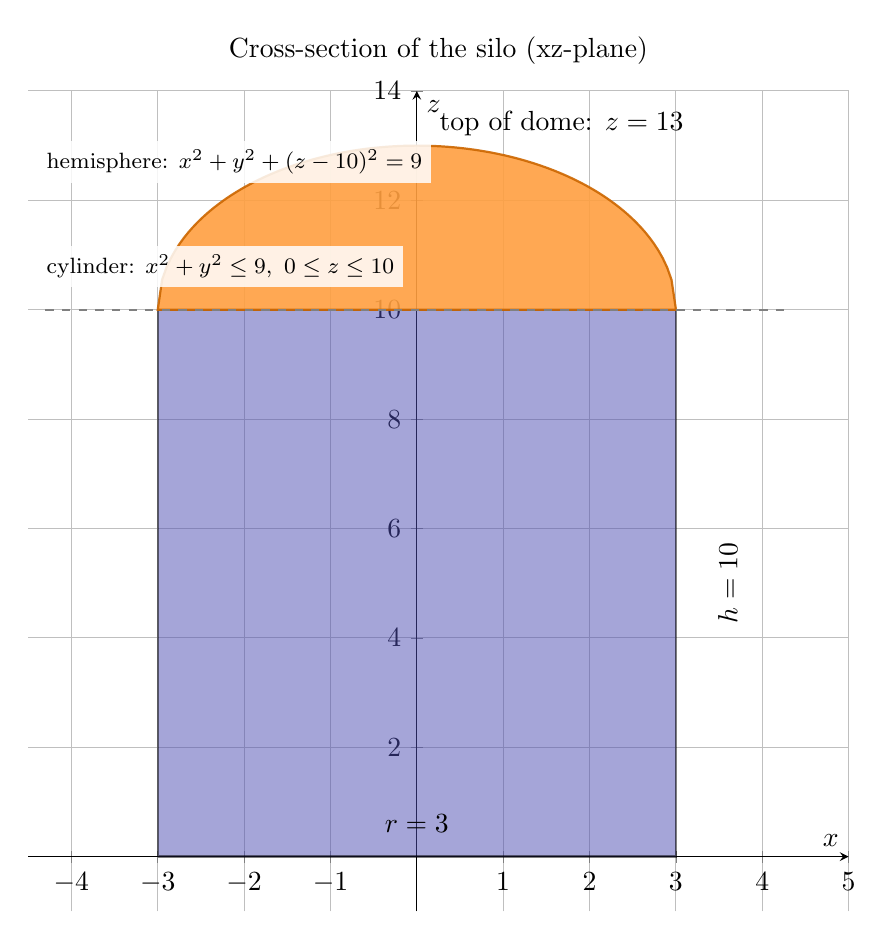
\begin{tikzpicture}
\begin{axis}[
    width=12cm, height=12cm,
    xlabel={$x$}, ylabel={$z$},
    xmin=-4.5, xmax=5, ymin=-1, ymax=14,
    title={Cross-section of the silo (xz-plane)},
    axis lines=middle,
    grid=major,
]
% Cylinder rectangle filled (blue)
\addplot[fill=blue!40!gray, opacity=0.5, draw=black, thick] coordinates {(-3,0) (3,0) (3,10) (-3,10) (-3,0)};
% Hemisphere fill: top arc closed along z = 10 (orange)
\addplot[fill=orange!75, opacity=0.9, draw=orange!80!black, thick, domain=-3:3, samples=120]
    {10 + sqrt(9 - x^2)} -- (axis cs:3,10) -- (axis cs:-3,10) -- cycle;
% Guide dashed line at z = 10
\addplot[dashed, gray, thick] coordinates {(-4.3,10) (4.3,10)};
% Annotations
\node at (axis cs:0,0.6) {$r=3$};
\node[rotate=90] at (axis cs:3.6,5) {$h=10$};
\node[anchor=west] at (axis cs:0.15,13.4) {top of dome: $z=13$};
\node[anchor=south west, font=\footnotesize, fill=white, opacity=0.85, text opacity=1] at (axis cs:-4.4,12.3) {hemisphere: $x^2+y^2+(z-10)^2=9$};
\node[anchor=south west, font=\footnotesize, fill=white, opacity=0.85, text opacity=1] at (axis cs:-4.4,10.4) {cylinder: $x^2+y^2\le 9,\ 0\le z\le 10$};
\end{axis}
\end{tikzpicture}
\end{document}
